\subsubsection{Functional Requirements}
\begin{itemize}
  \item The system shall tag a car avaible again if a related reservation is deleted
  \item The system shall not apply any charge if the reservation is deleted before expiration
\end{itemize}


\subsubsection{Scenario 1}
Michael is in a hurry because he has a meeting downtown in 20 minutes, he is really late and after locating a PowerEnJoy car he submits a reservation. He is about to unlock the car when he hears someone calling his name, a collegue recognized him and stopped to offer him a ride. Michael accepts but he immediately cancels his reservation in order to avoid the expiration fine and allow other users to take advantage of the service. The system processed his request and now the car is available again. 


\subsubsection{Mockups}
\begin{figure}[!ht]
  \centering
  \vspace{0.2cm}
  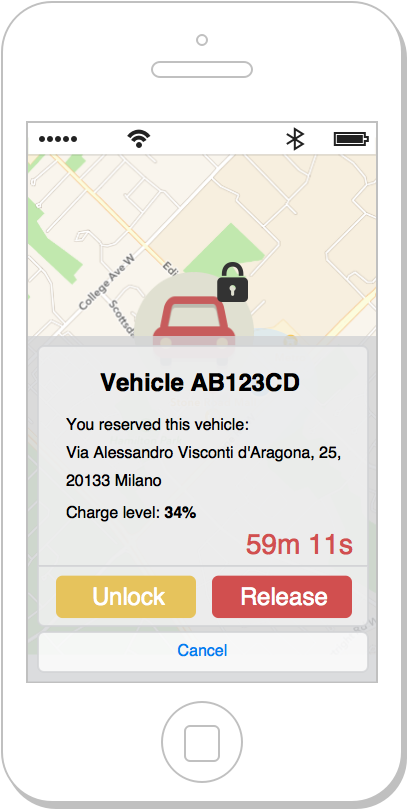
\includegraphics[width=0.25\textwidth]{/RASD/System_Functions/delete_reservation_mockup}\\
  \vspace{0.4cm}
  %\caption{Mockup for the reservation deletion mobile page} 
  \label{fig:delete_reservation} 
\end{figure}
% maybe home page mockup here 


\subsubsection{Use-case table}
\begin{center}
  \begin{tabular}{ l | p{10cm} }
    \hline
    Actors & User\\ \hline
    Goal & G\ref{itm:goal-reservation}\\ \hline
    Entry conditions & The User has previously reserved a vehicle and wants to delete the reservation
     \\ \hline
    Flow of events &
    \begin{itemize} 
      \item The User opens the application 
      \item The Users visualizes in his home page the active reservation
      \item The User clicks "Delete" in order to release his reservation
      \item The system processes his request and updates the car status
      \item The system loads the User's homepage.
    \end{itemize} \\ \hline
    Exit conditions & The User is in his homepage but his last reservation has been deleted and the vehicle is free again \\ \hline
  	Exceptions & 
    \begin{itemize}
      %we assume here that the system reacts in real time in case of expiration and so a deletion cannot be requested
      \item The system is not able to complete the operation due to some internal issues or connection broken (the system signals a ConnectionFailure). % modifiable exceptions names
    \end{itemize} \\ \hline
  \end{tabular}
\end{center}


\subsubsection{Sequence diagram}
\begin{figure}[!ht]
  \centering
  \vspace{0.2cm}
  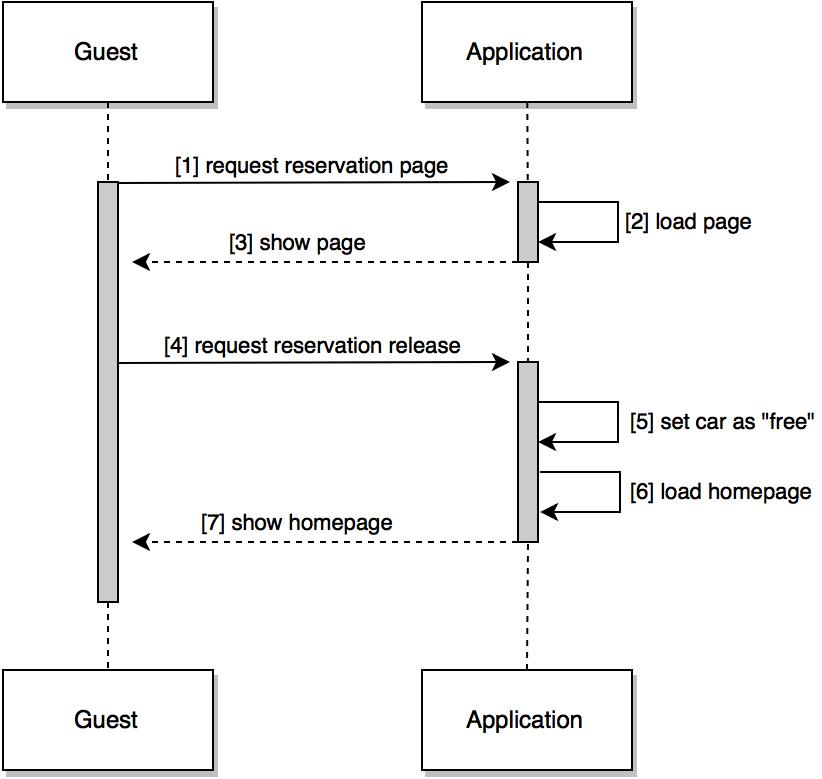
\includegraphics[width=0.6\textwidth]{/RASD/System_Functions/delete_reservation_sequence}\\
  \vspace{0.4cm}
  %\caption{Sequence diagram for the reservation release procedure} 
  \label{fig:delete_reservation_sequence} 
\end{figure}
